% Editable LaTeX conversion of the accepted V14 scientific report.
% All report paragraphs, tables, figures, references and appendices are retained.
% One obsolete affiliation-status sentence is corrected; equations are typeset.
\documentclass[a4paper,10pt]{article}
\usepackage[T1]{fontenc}
\usepackage[utf8]{inputenc}
\usepackage{mathptmx,amsmath,amssymb,graphicx,booktabs,array,tabularx}
\usepackage[a4paper,left=14.8mm,right=14.8mm,top=12.4mm,bottom=14mm,footskip=7mm]{geometry}
\usepackage{xcolor,microtype,xurl,hyperref}
\definecolor{ink}{HTML}{263B35}
\definecolor{accent}{HTML}{24656B}
\hypersetup{colorlinks=true,urlcolor=accent,linkcolor=accent,pdftitle={When a Local Pricing Guard Is Not a Welfare Promise},pdfauthor={Mohammadpayam Taebi}}
\setlength{\parindent}{0pt}
\setlength{\parskip}{5.4pt}
\setlength{\tabcolsep}{4pt}
\renewcommand{\arraystretch}{1.08}
\setlength{\emergencystretch}{2em}
\newcommand{\reportheading}[1]{\par\vspace{5pt}{\large\bfseries\color{ink}#1}\par\vspace{2pt}}
\newcommand{\reportcaption}[1]{{\fontsize{8.4}{10.2}\selectfont #1\par}\vspace{3pt}}
\begin{document}
\fontsize{10.6}{13.2}\selectfont
\noindent\textcolor{ink}{\rule{\linewidth}{1.6pt}}


% Source section 1: Title, abstract and question

\begin{center}\vspace*{1mm}{\fontsize{21}{24}\selectfont\bfseries\color{ink}When a Local Pricing Guard\\
Is Not a Welfare Promise}\end{center}

\begin{center}Finite precision, continuing intervention and adaptive behavior in a bounded logit market\end{center}

\noindent\textcolor{ink}{\rule{\linewidth}{0.5pt}}

\begin{center}Mohammadpayam Taebi\\
The Chinese University of Hong Kong (CUHK)\\
AI Collusion Research Sprint \textperiodcentered{} 26 October 2026\end{center}

\begin{center}Sprint organizers: Apart Research \textperiodcentered{} Poseidon Research \textperiodcentered{} AE Studio\end{center}

{\fontsize{9.4}{11.6}\selectfont \textbf{Abstract.} A local pricing rule can improve observed customer benefit without guaranteeing its target. We study a bounded logit duopoly where a guard permits near-best immediate profit against the rival's previous price. A one-time cap appears protective in a coarse game, but the continuous worst long-run benefit is 66.272, below the unchanged 95\% target of 68.513. An attainable price envelope characterizes continuing use of the same cap. A funded calendar minimizes worst-path cap frequency within causal cap-or-guard controllers protecting every activation prefix; base effective-continuous frequency falls about 7.29\% from its best fixed period. Separate finite and continuous calculations retain 120 target labels. An earlier 192-run learning study has unequal clock capacities. A prospectively frozen 24-run follow-up matches five phases and dense memory: recurring limits improve final frozen-cycle benefit by 0.956 units, with all twelve paired differences positive. A further twelve-run reference removes the post-startup guard over the original grid at the same budget. Customer benefit falls in all twelve pairs, by 12.733 units on average; not every shop gains against static Nash. Separately authored replay checks every round of both follow-ups. Static anchors and a 48-label frozen-partner audit keep observed behavior distinct from equilibrium and individual incentives. These finite-budget results combine learning and execution constraints and do not establish convergence, collusion prevention or intent. The contribution is a model-specific guarantee audit, controlled behavioral comparisons and a graphical game using established methods.\par}

\reportheading{1 The problem: a local check and a long-run promise}

Two shops choose prices simultaneously. Each wants its own profit. An external guard checks a proposed price against the other shop's \emph{last completed} price. Passing that check says little by itself about what customers obtain after many executions. We ask what customer-benefit promise survives a one-time handover back to this guard, and what continuing control is needed for a stronger promise.
\par

A cap is a real market round: it limits both executed prices, makes purchases and earns profit and customer surplus. It is not a free reset of a chart. Our human game deliberately lets a coordinator choose both shops' prices. That illustrates permitted behavior; it does not establish independent collusion or supply human experimental data.
\par

{\fontsize{9.4}{11.6}\selectfont \textbf{What is added.} The linked sprint starter already provides replacement, history, objective and checkpoint-branch experiments [1]. We audit an explicit external price rule: precision, attainable adverse behavior, same-cap timing, model reserve, local learning and individual responses against saved learned partners. Known control and learning methods are credited below; priority for these ingredients is not claimed.\par}

\clearpage

% Source section 2: Model and quantifiers

\reportheading{2 A self-contained game and the scope of each claim}

There are B potential buyers, two symmetric inside goods of quality v and cost c, an outside option of normalized utility zero, and taste scale $\mu>0$. At executed physical prices $p_A,p_B$, let $e_i=\exp((v-p_i)/\mu)$. Expected demand, private profit and customer surplus are:
\par

\begin{align*}
D_i &= \frac{B e_i}{1+e_A+e_B}, & R_i &=(p_i-c)D_i,\\
C(p_A,p_B)&=B\mu\log(1+e_A+e_B), & e_i&=\exp((v-p_i)/\mu).
\end{align*}

The base calibration is B=100, v=2, c=1 and $\mu$=0.25. Its inherited bounded physical price domain is approximately [1.427721, 1.970186]. The inherited cap is held exactly at its saved numerical value $p_{\rm cap}$=1.4664687420450921; it is not moved to a different continuous Nash price when timing changes. The original 15-quote reference gives cap customer benefit approximately 72.119. The unchanged relaxed 95\% target F is approximately 68.513, stored as an absolute numerical threshold. Different experiments do not quietly redefine this target.
\par

Let q be the rival's previous completed price. The guard permits every price in the bounded domain whose immediate expected profit is within $\epsilon$ of the best immediate profit available against q:
\par

\begin{align*}
\mathcal S(q)&=\{p:\max_z R(z,q)-R(p,q)\leq\epsilon+\tau\}, & U(q)&=\max\mathcal S(q).
\end{align*}

Epsilon=0.1 in the base mask; the learner sensitivity uses $\epsilon$=0.05. Tau is the inherited $10^{-12}$ numerical comparison allowance. This is a lagged one-step modeled profit-loss rule, not calibrated regret and not loss against the rival's hidden current action. Both sellers are externally constrained; they may coordinate, randomize or use arbitrary history within the legal sets when we state an \emph{all-policy} guarantee.
\par

\reportcaption{Table 1. Four evidence types and their distinct scopes.}

{\fontsize{9}{10.8}\selectfont\noindent\begin{tabular}{@{}>{\raggedright\arraybackslash}p{0.2036660\dimexpr\linewidth-24pt\relax}>{\raggedright\arraybackslash}p{0.3951120\dimexpr\linewidth-24pt\relax}>{\raggedright\arraybackslash}p{0.4012220\dimexpr\linewidth-24pt\relax}@{}}\toprule
\textbf{Object} & \textbf{What is computed} & \textbf{What it does not establish}\\\midrule
Saved finite game & Exact rational comparisons on the saved binary64 payoff weights and legal masks. & Exact-real logit inequalities or grid-invariant protection.\\
Validated continuous model & Directed Decimal interval bounds for imported real constants under checked monotonicity and contraction conditions. & An independent transcendental backend or empirical market validity.\\
Learning behavior & Fixed-budget local Q-learning, paired seeds, saved-policy continuation and visit support. & Convergence, equilibrium, intent, or LLM behavior.\\
Frozen-partner incentives & Exact achieved discounted values and a best-response upper bound from saved histories. & Discoverability, resumed learning or every-state equilibrium.\\
\bottomrule\end{tabular}\par}\vspace{3pt}

{\fontsize{9.4}{11.6}\selectfont In the graphical cap game a saved 61-quote base mesh is augmented by the exact old cap, prioritizing that quote over a nearby mesh quote. The two learner masks each have 62 choices. These are separate numerical games from the original 15-quote and refinement meshes; a continuous period is independently checked in the finite game before any finite guarantee is asserted.\par}

{\fontsize{9.4}{11.6}\selectfont Finite masks inherit the binary64-rounded $\epsilon+\tau$ comparator. Continuous validation separately treats imported constants as exact reals and reports nominal/effective allowances. ``Continuous limit'' describes the model result, not a proof that bit-level JavaScript mask rounding vanishes.\par}

\reportheading{Different questions, different outcomes}

An all-policy floor concerns every allowed path. A training average concerns the actual exploratory updates. A frozen continuation stops updates and exploration and follows the saved greedy choices. These answer different questions, and the paper and game keep them visible separately.
\par

\clearpage

% Source section 3: Price precision and recurring protection

\reportheading{3 The handover promise weakens with richer prices}

Under the verified base continuous assumptions, U is monotone and contractive on the inherited interval. It has a unique fixed point $q^\star$. Prices on every permitted path are bounded above by iterating U, and the upper choices themselves are permitted. Since customer surplus decreases in either price, $C^\star$=$C(q^\star,q^\star)$ is a tight worst long-run floor. This does not require every permitted price path to converge.
\par

\begin{center}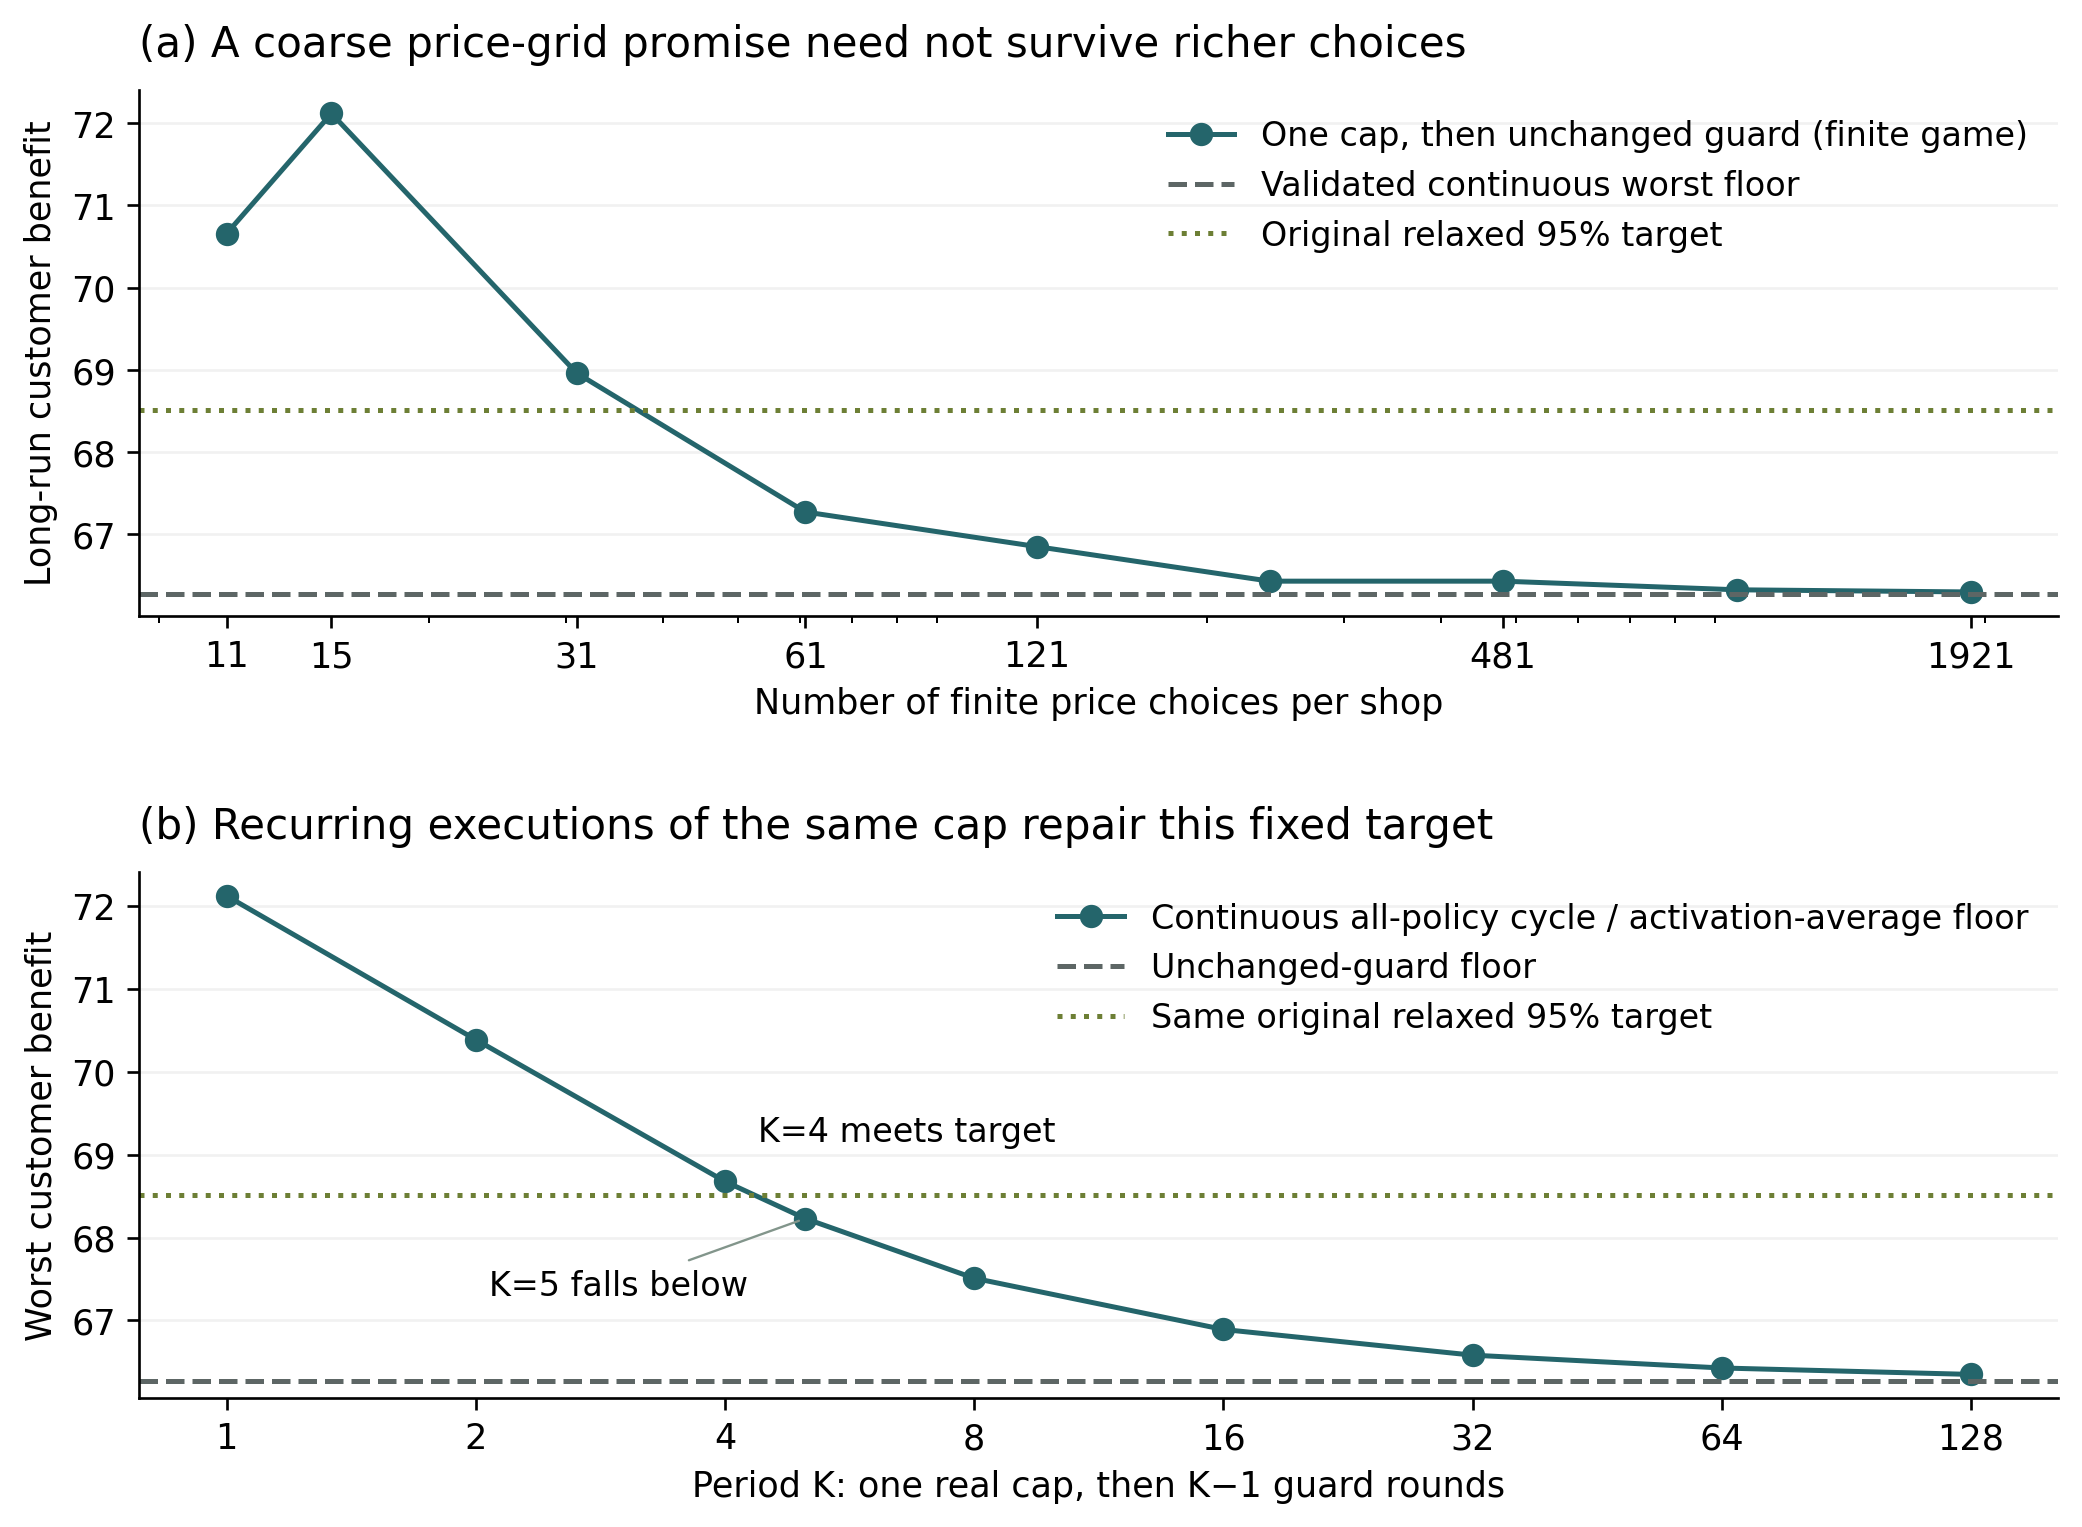
\includegraphics[width=0.94\linewidth]{images/precision-and-timing.png}\end{center}

\reportcaption{Figure 1. Base condition. (a) Saved finite one-cap floors at the predeclared mesh sizes and the validated continuous floor. Refinement is not monotone across all coarse meshes; the 11-choice case is already worse than the 15-choice case. (b) A different object: validated continuous recurring-cap floors $G_K$, with the same old physical cap and unchanged target. These plots show all-policy capacity, not observed learning.}

{\fontsize{9.4}{11.6}\selectfont The 15-choice one-cap floor is about 72.119, while the 1,921-choice diagnostic is about 66.298 and the continuous limit is 66.272. The original target is 68.513. A finite initializer changes a transient; it cannot raise the asymptotic continuous floor above $C^\star$ when the unchanged guard then runs forever.\par}

\reportheading{A tight repair within the fixed-period family}

Keep physical price units: let $a_0$=$p_{\rm cap}$ and $a_{j+1}=U(a_j)$, and put $r_j=C(a_j,a_j)$. The actual first cap is phase 0; K-1 guard rounds follow. The worst repeated cycle is attained by both shops choosing their maximum legal quote:
\par

\[G_K=\frac{1}{K}\sum_{j=0}^{K-1}r_j.\]

{\fontsize{9.4}{11.6}\selectfont The verified sequence $r_j$ decreases, so every cap-first finite running average is at least $G_K$; a later individual round can still fall below it. The base target permits K=4 ($G_4$ about 68.676), but K=5 fails (about 68.229). Both 99\% and 100\% reference targets need K=1 in these audited labels. ``Largest safe K'' means largest \emph{fixed integer period in this same-cap family}. Frequency 1/K counts rule applications, not economic cost, changed quotes or autonomy.\par}

\clearpage

% Source section 4: Mixed timing and the integer-period restriction

\reportheading{4 Can mixed gaps improve the same protection promise?}

Let $S_\ell$ sum the first l adverse rewards and K be the largest safe fixed period. A K-round block banks $a=S_K-KF\geq0$; a K+1 block spends -b, where b=$S_{K+1}-(K+1)F<0$. Fund that entire debt before using the longer gap. Concavity then protects every activation prefix, including one ending inside a block.
\par

\[p=\frac{a}{a-b},\qquad \text{minimum worst-path cap-rule rate}=\frac{1}{K+p}.\]

{\fontsize{9.4}{11.6}\selectfont The feasible maximum-price response and Jensen inequality, including the last partial gap, force this lower rate for any causal two-mode controller. Bounded funded credit attains it. This is asymptotic minimax optimality within the stated family; sliding windows and pointwise minimum cap counts are different promises. The guard remains active between caps. The methods have close prior art [9--12]; the full conditional proof is in MIXED\_TIMING\_THEORY.md.\par}

\begin{center}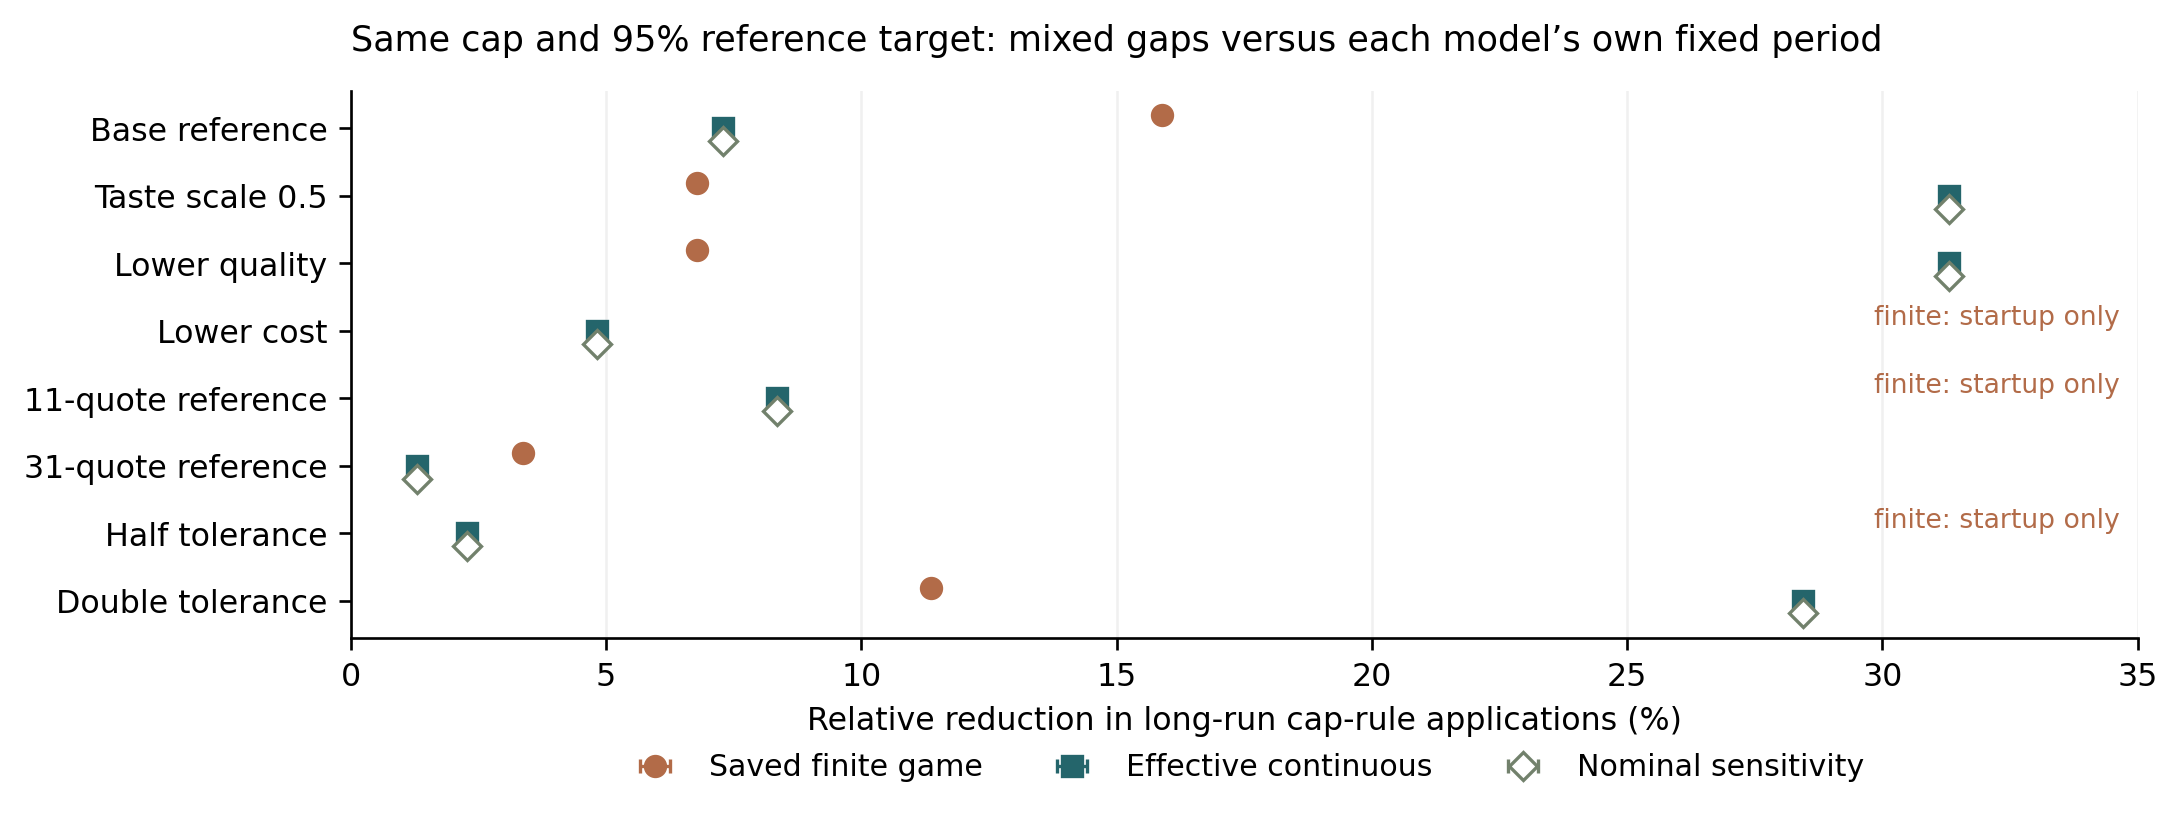
\includegraphics[width=0.94\linewidth]{images/timing-frontier.png}\end{center}

\reportcaption{Figure 2. Prospectively selected 95\% target, all eight scenarios and three model interpretations. Reductions use each record's own best fixed period. Points are constructed feasible reductions; continuous enclosures are too narrow to resolve graphically but remain nonzero. Startup-only rows have no largest fixed comparator and are labeled rather than plotted as zero savings. Reference-grid labels identify inherited conditions; finite games have 61/62 choices.}

\reportcaption{Table 2. Same physical cap and target, different numerical models. Rates are long-run cap applications per execution; decimals are approximate.}

{\fontsize{9}{10.8}\selectfont\noindent\begin{tabular}{@{}>{\raggedright\arraybackslash}p{0.2179226\dimexpr\linewidth-48pt\relax}>{\raggedright\arraybackslash}p{0.0753564\dimexpr\linewidth-48pt\relax}>{\raggedright\arraybackslash}p{0.1425662\dimexpr\linewidth-48pt\relax}>{\raggedright\arraybackslash}p{0.1894094\dimexpr\linewidth-48pt\relax}>{\raggedright\arraybackslash}p{0.1670061\dimexpr\linewidth-48pt\relax}>{\raggedright\arraybackslash}p{0.2077393\dimexpr\linewidth-48pt\relax}@{}}\toprule
\textbf{Base 95\% model} & \textbf{Own K} & \textbf{Fixed rate} & \textbf{Constructed rate} & \textbf{Reduction} & \textbf{First long round}\\\midrule
Saved finite & 5 & 0.200000 & 0.168238223 & 15.8809\% & 6\\
Effective continuous & 4 & 0.250000 & 0.231782998 & 7.2868\% & 13\\
\bottomrule\end{tabular}\par}\vspace{3pt}

{\fontsize{9.4}{11.6}\selectfont All 120 labels remain: 40 finite give 10 startup-only cases and 30 exact adjacent optima; 80 continuous give 14 startup-only cases and 66 enclosures. All 96 adjacent savings are positive because a>0 here, not because 96 empirical trials succeeded. Every continuous rate enclosure has nonzero width (maximum below $4.19\times10^{-28}$). Twelve finite first-long times exceed the 256-round preview; 26 continuous times exceed 64 rounds. At the 100\% target, first long gaps require millions of executions. The 192-run learner study below keeps its old fixed clocks; it supplies no behavior under this new calendar.\par}

\clearpage

% Source section 5: Adaptive learners and matched architecture

\reportheading{5 Controlled learning comparisons}

The earlier study retains 192 runs: two saved 62-price masks in one economic calibration, four schedules, two Q initializations and twelve whole-market seeds. Each run has two million simultaneous rounds and 1M/2M checkpoints. The startup controller has two phase labels while recurring controllers have K; equal rounds therefore do not match representation capacity. That study remains informative about its declared systems, but cannot isolate cap frequency or clock capacity.
\par

Both firms use established masked tabular Q-learning, own expected profit and private score tables. They choose simultaneously from the last completed price pair. Next-state bootstrap maxima for both firms are captured before either current update; exact ties choose the smallest original quote index:
\par

\[Q(s,a)\leftarrow Q(s,a)+0.1\Bigl[R_{\rm own}+0.95\max_{a'\text{ legal}}Q(s',a')-Q(s,a)\Bigr].\]

\reportcaption{Table 3. Separate 24-run matched-clock follow-up; no old run is relabeled or replaced.}

{\fontsize{9}{10.8}\selectfont\noindent\begin{tabular}{@{}>{\raggedright\arraybackslash}p{0.2179226\dimexpr\linewidth-16pt\relax}>{\raggedright\arraybackslash}p{0.7820774\dimexpr\linewidth-16pt\relax}@{}}\toprule
\textbf{New matched factor} & \textbf{Prospectively fixed values}\\\midrule
Physical game & Same original-tolerance 62-price table, cap and guard; no new payoff enumeration.\\
Shared public clock & 0 -> 1 -> 2 -> 3 -> 4 -> 1. Phase 0 occurs once; phases 1-4 recur in both arms.\\
Only rule difference & Startup caps only phase 0. Recurring caps phases 0 and 4; all other phases use the original guard.\\
Private allocation & Each firm has 5*62\textasciicircum{}3 = 1,191,640 binary64 Q cells and equal uint32 visit-count capacity, initialized to positive zero.\\
Budget and streams & 12 intentionally reused seed IDs, both arms, 2M rounds. Paired private xoshiro128** streams consume two words per firm per round.\\
Learning and endpoints & Alpha 0.1; binary64 gamma 0.95; exploration 1 to 0.01. Checkpoints 1M/2M; final actual-history frozen-cycle customer benefit is primary.\\
\bottomrule\end{tabular}\par}\vspace{3pt}

At both checkpoints the NEXT phase is 4: guard for startup, cap for recurring. Keep each arm's actual price history and full cap-state memory; do not add a fresh phase 0 cap. Both arrays have the same allocated capacity, while legal actions, experience and visits differ. Four recurrent clock labels also let the startup learner condition on public time. The clock closes controller state; opponent adaptation still makes each firm's learning problem nonstationary.
\par

{\fontsize{9.4}{11.6}\selectfont This contrast measures the total effect of changing ongoing legal control during training and frozen evaluation. It does not isolate formation from enforcement or explain how much of the older gap came from representation. The K=4 rhythm follows the old learned stratum; it is distinct from finite K=5 or the later funded calendar. All twelve exact paired rows and their exact arithmetic mean are planned; any missing final pair nulls that mean. No new CI or p-value is planned.\par}

{\fontsize{9.4}{11.6}\selectfont A separate prospectively fixed reference adds twelve new runs: after the same one-time cap, every original price is legal in phases 1 through 4. Physical rewards, clock labels, dense allocation, zero initialization, paired streams and 2M budget match the accepted startup guard. This removes the post-startup guard during training and frozen evaluation together. Broader legal action sets also change visits per action; equal budget is not equal learning difficulty. All 35 sources and 812 inputs are frozen before the actual reference runs.\par}

\clearpage

% Source section 6: Earlier comparisons and matched-clock findings

\reportheading{6 Matched-clock findings and earlier context}

\reportcaption{Table 4. Earlier 192-run study: selected95 minus startup actual-terminal cycle benefit. Each stratum has 12 paired seeds; approximate marginal seed-resample intervals are not market uncertainty or causal frequency estimates.}

{\fontsize{9}{10.8}\selectfont\noindent\begin{tabular}{@{}>{\raggedright\arraybackslash}p{0.1405295\dimexpr\linewidth-40pt\relax}>{\raggedright\arraybackslash}p{0.1588595\dimexpr\linewidth-40pt\relax}>{\raggedright\arraybackslash}p{0.1934827\dimexpr\linewidth-40pt\relax}>{\raggedright\arraybackslash}p{0.2505092\dimexpr\linewidth-40pt\relax}>{\raggedright\arraybackslash}p{0.2566191\dimexpr\linewidth-40pt\relax}@{}}\toprule
\textbf{Tolerance} & \textbf{Scores} & \textbf{Mean difference} & \textbf{All-seed range} & \textbf{Marginal 95\% interval}\\\midrule
Original & zero & +2.480 & +2.031 to +2.978 & +2.317 to +2.638\\
Original & optimistic & +2.391 & +1.663 to +5.135 & +1.850 to +3.160\\
Half & zero & +2.457 & +2.158 to +2.664 & +2.377 to +2.536\\
Half & optimistic & +2.946 & +1.998 to +3.517 & +2.657 to +3.197\\
\bottomrule\end{tabular}\par}\vspace{3pt}

{\fontsize{9.4}{11.6}\selectfont The older four-stratum means range from 2.391 to 2.946 units, with 48/48 positive rows. Its full training trajectory was not independently replayed; saved checkpoints, graphs, sampled updates and cloned probes were checked. The old and new systems are different versions, not interchangeable independent replications.\par}

\begin{center}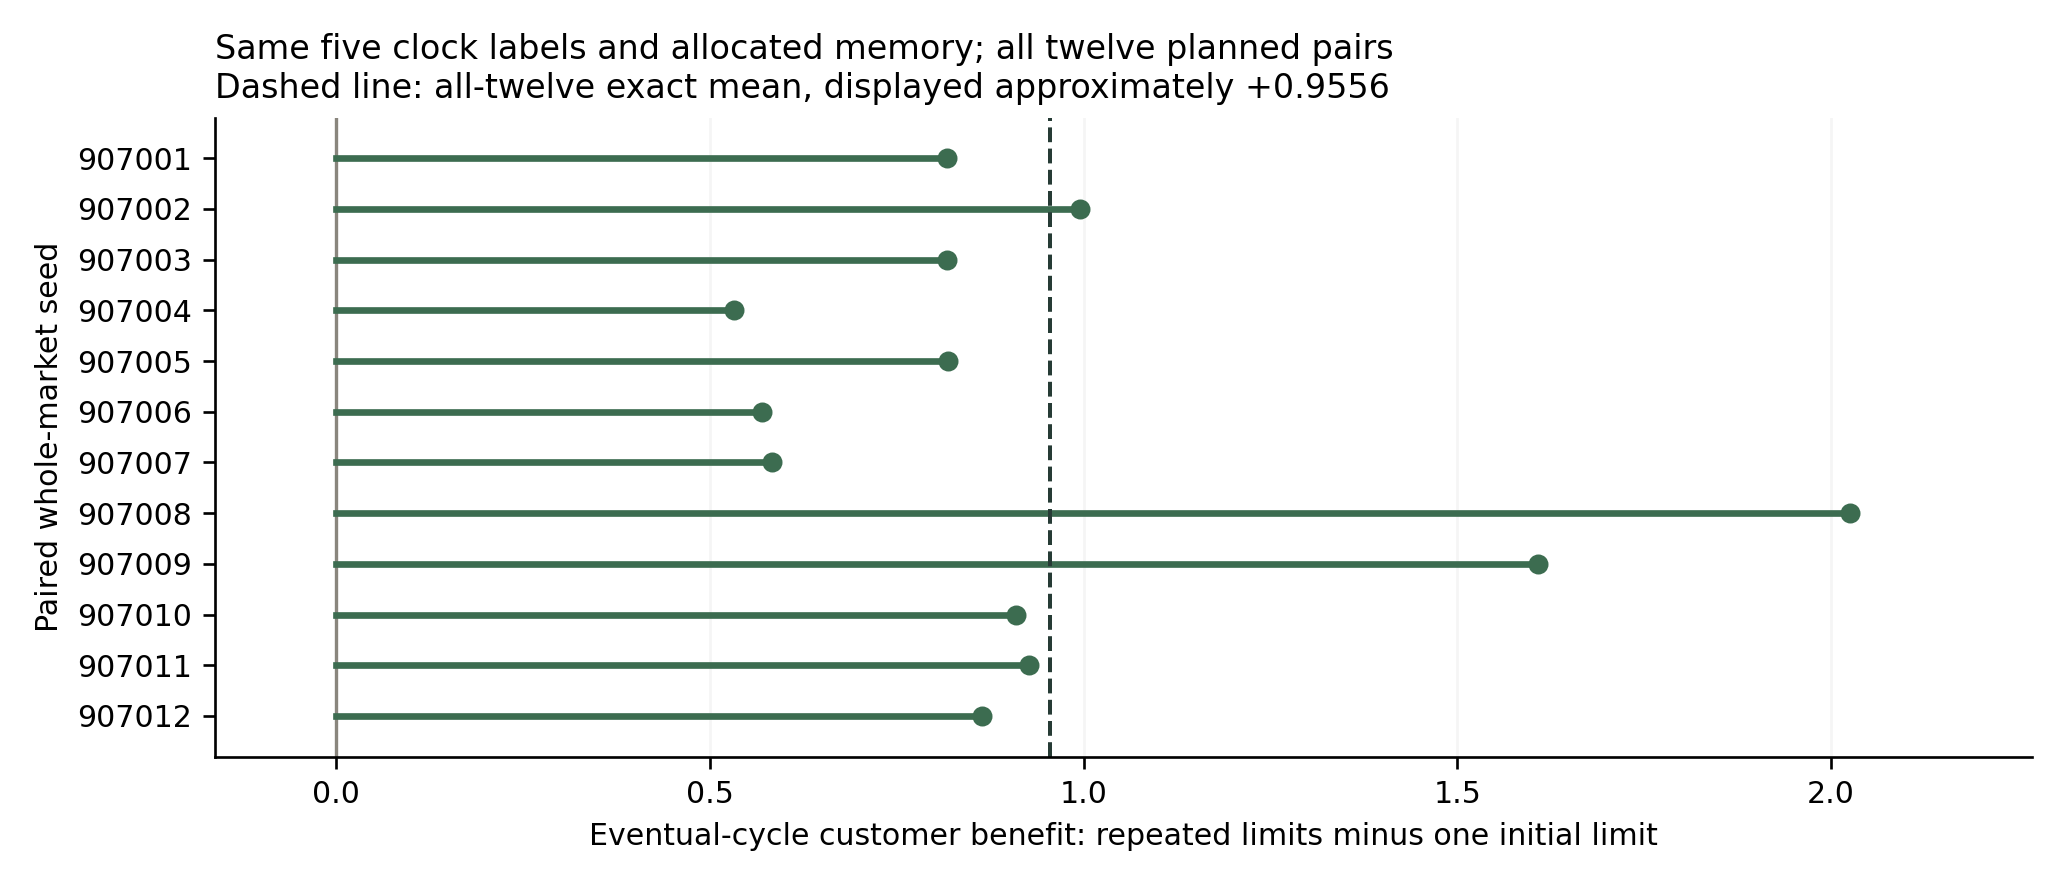
\includegraphics[width=0.94\linewidth]{images/matched-clock-paired.png}\end{center}

\reportcaption{Figure 3. Separate 24-run matched architecture: every final actual-terminal recurring-minus-startup cycle-benefit difference. Solid segments begin at zero; dashed vertical line is the planned all-twelve mean. All exact rows, including zero, reversed or unavailable outcomes, remain in the evidence. These are twelve whole-market seed contrasts with paired treatments in one saved finite model, with no confidence interval.}

The new planned mean is 0.955595 customer-benefit units. Accepted pairs: 12/12; exact signs: 12 positive, 0 zero and 0 negative. Display decimals are approximate. Equal clock labels and allocated capacity therefore retain a positive difference in this execution; this is not proof of convergence or a causal explanation of the older larger gap.
\par

{\fontsize{9.4}{11.6}\selectfont Independent full replay accepted 48/48 checkpoints and 24/24 final endpoints, with 0 execution failures. It reexecuted 48,000,000 rounds. Aggregate full-replay and checkpoint-completeness flags are True and True; these concern only the new 24 runs. Every one of the 24 cycle-benefit endpoints changes between 1M and 2M, so these checkpoints give no convergence claim. Training-tail averages and arbitrary-state graph diagnostics remain secondary and separate from eventual-cycle means.\par}

\clearpage

% Source section 7: Full-grid capability reference

\reportheading{7 What changes when the guard is removed?}

The twelve new full-grid continuations reuse the accepted startup-guard comparators, not their training. Both begin with the same real cap. Only later legal price choices change. Each final policy pair continues its actual history and NEXT phase 4, with no fresh cap, exploration or updates.
\par

\begin{center}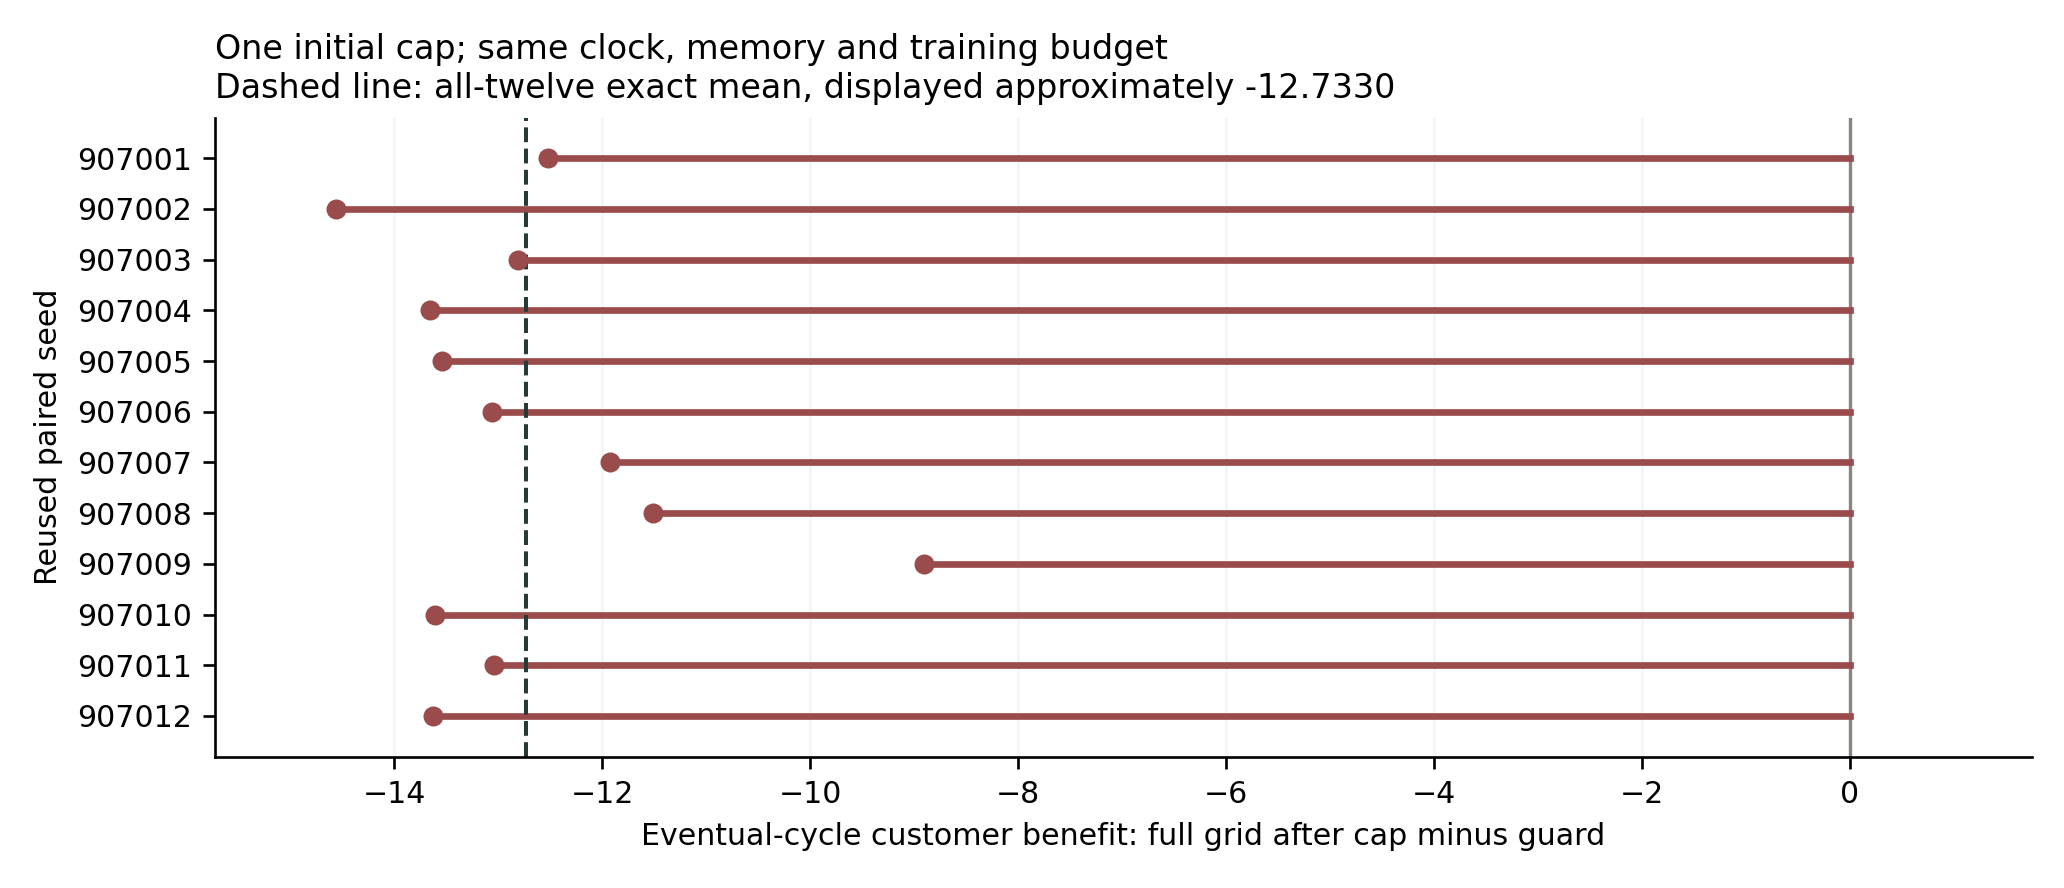
\includegraphics[width=0.94\linewidth]{images/guard-reference-paired.png}\end{center}

\reportcaption{Figure 4. All twelve registered full-grid-minus-guard eventual-cycle customer-benefit differences. Every signed row is retained in seed order; the dashed line is the exact all-twelve mean displayed approximately. Negative differences favor the guard. These are paired streams in one saved finite game, with no confidence interval.}

The planned mean difference is -12.733 customer-benefit units; signs are 0 positive, 0 zero and 12 negative. Mean benefit is 57.137449 for full-grid continuation and 69.870422 for startup guard. The guard therefore meaningfully improves these learners' realized benefit while the earlier theory still rejects a stronger all-policy target promise.
\par

\reportcaption{Table 5. Every retained static pair on the original full simultaneous grid; decimals approximate, joint objectives exact. These are not equilibria of the learned history-dependent policies.}

{\fontsize{9}{10.8}\selectfont\noindent\begin{tabular}{@{}>{\raggedright\arraybackslash}p{0.1384929\dimexpr\linewidth-64pt\relax}>{\raggedright\arraybackslash}p{0.0936864\dimexpr\linewidth-64pt\relax}>{\raggedright\arraybackslash}p{0.1201629\dimexpr\linewidth-64pt\relax}>{\raggedright\arraybackslash}p{0.1201629\dimexpr\linewidth-64pt\relax}>{\raggedright\arraybackslash}p{0.1262729\dimexpr\linewidth-64pt\relax}>{\raggedright\arraybackslash}p{0.1262729\dimexpr\linewidth-64pt\relax}>{\raggedright\arraybackslash}p{0.1303462\dimexpr\linewidth-64pt\relax}>{\raggedright\arraybackslash}p{0.1446029\dimexpr\linewidth-64pt\relax}@{}}\toprule
\textbf{Static anchor} & \textbf{A/B indices} & \textbf{Price A} & \textbf{Price B} & \textbf{Profit A} & \textbf{Profit B} & \textbf{Joint profit} & \textbf{Benefit}\\\midrule
Static pure Nash & 6 / 6 & 1.472927 & 1.472927 & 22.293 & 22.293 & 44.585 & 71.510\\
Joint-profit maximum & 56 / 56 & 1.924981 & 1.924981 & 33.749 & 33.749 & 67.498 & 32.708\\
\bottomrule\end{tabular}\par}\vspace{3pt}

{\fontsize{9.4}{11.6}\selectfont All new final-cycle states and chosen actions had training support. Cycle customer benefit changes between 1M and 2M in 3/12 runs; unchanged checkpoints are not convergence evidence. Against static Nash, 23/24 individual cycle profits are higher, but seed 907009 Shop B earns 19.1434 versus 22.2927. Both shops do not always gain. The reference remains below the joint-profit maximum and does not establish stable collusion, punishment, intent or equilibrium.\par}

\clearpage

% Source section 8: Interpretation, contribution and access

\reportheading{8 What this adds, and what remains open}

The strongest result is about \emph{the scope of a protection promise}. A coarse finite game can give a reassuring one-cap result while a richer price interface admits worse allowed continuations. The continuous upper envelope explains the limit and gives an attainable worst cycle when the same physical cap is repeated. Calibration reserve and unilateral incentives identify different boundaries: model error can consume the old absolute target, while a worst permitted script need not be individually attractive.
\par

The learner study adds behavior under a precisely declared controller, without replacing the all-policy proof by a favorable simulation. Its outcomes remain conditional on two masks, one calibration, chosen hyperparameters, finite budget and private-score initializations. Neither high prices nor a quiet frozen cycle establishes collusion, punishment, intent or equilibrium. The new learned-partner audit establishes modest unilateral opportunities against fixed saved policies, not mutual adaptation or punishment. The matched follow-up addresses clock labels and allocated memory in one stratum; the full-grid reference separately measures post-startup support removal. The new full-original-grid reference closes one capability-reference gap under the same initial cap and budget. Further work needs learning sensitivity, separated training/evaluation interventions and continued adaptation. It does not remove the finite price domain or establish capability under other budgets.
\par

\reportheading{Relation to prior work and the sprint starter}

Calvano et al. study profit-seeking learning and algorithmic pricing [2]. Eschenbaum et al. examine robustness, replacement and continued adaptation [3], and the sprint starter already branches histories, models and objectives [1]. Alshiekh et al. define action restriction and shielding, including reward credit and the need for persistent protection [5]. Brero et al. design ongoing platform interventions for consumer benefit [6]. Hartline et al. study a different, calibrated-regret regulation framework [7]. Periodic resetting and renewal-ratio control are established [8,9]. Lopes de Moraes and De Losso directly audit learned pricing incentives [4]. None should be repackaged here as our invention.
\par

Our limited addition is a linked guarantee-capacity case: precision, a fixed physical cap, restricted minimax timing, bounded demand reserve, adaptive observations and certified learned-partner responses keep distinct quantifiers. Frozen-policy response MDPs are already explicit in [4], Sections3.2(iv),4.5; our standard Bellman bound is not a new algorithm. Adjacent timing mixtures already occur in Sun and Cyr [10]; uniform cumulative safety budgets appear in conservative bandits [11,12]. Our pricing-envelope reduction and validated comparison apply these ideas. The mixed result covers the same two actuators, not every intervention, cap strength or economic cost. No broad novelty or empirical-market superiority is established.
\par

\reportheading{An accessible game, with evidence behind each view}

Start at http://127.0.0.1:3003/. The two-shop challenges let a human choose both permitted quotes, see actual cap executions and separate earned customer benefit from a guaranteed buffer. The mixed-calendar page explains how earlier credit funds a longer gap. The one-shop profit challenge uses a public script and exact block score; the learner page reveals stored executions. The one-shop continuation lets a person choose against a saved deterministic learner. The /reference page distinguishes watching saved shops from choosing human prices and shows all twelve guard-removal contrasts, static anchors and individual profits. The earlier paired /matched replay advances two accepted final worlds together, with equal-clock graphics, all twelve signed differences, undo and restart; finite earned scores stay separate from complete cycles and audited infinite values. These are explanatory artifacts and developer-tested controls, not a human usability study.
\par

\reportheading{Reproduction}

{\fontsize{9.4}{11.6}\selectfont Open /reference to watch the saved guard/full-grid comparison, or /recurring to choose both prices. README records the audit/build commands, pinned Python 3.13 and archive roles. Full-round replay covers the matched 24 and reference 12 runs; the earlier 192 retain their narrower audit. The smaller viewer omits large checkpoints and names the full evidence hash.\par}

{\fontsize{9.4}{11.6}\selectfont Verification checks are coverage evidence, not experimental sample size. The exact finite calculations share their economic model; the continuous checkers use separate directed-interval code but the same Decimal transcendental backend. Independent AI-agent review does not substitute for external human peer review.\par}

\clearpage

% Source section 9: References

\reportheading{References}

{\fontsize{9.4}{11.6}\selectfont [1] Poseidon Research. Collusion hackathon starter, llm-cartel, 2026. Replacement, history, objective and checkpoint-branch code.\\
\href{https://github.com/poseidon-research/collusion_hackathon/tree/main/llm-cartel}{https://github.com/poseidon-research/collusion\_hackathon/tree/main/llm-cartel}\par}

{\fontsize{9.4}{11.6}\selectfont [2] E. Calvano, G. Calzolari, V. Denicolo and S. Pastorello. Artificial Intelligence, Algorithmic Pricing, and Collusion. American Economic Review 110(10), 3267-3297, 2020.\\
\href{https://doi.org/10.1257/aer.20190623}{https://doi.org/10.1257/aer.20190623}\par}

{\fontsize{9.4}{11.6}\selectfont [3] N. Eschenbaum, F. Mellgren and P. Zahn. Robust Algorithmic Collusion. arXiv:2201.00345,2022.\\
\href{https://arxiv.org/abs/2201.00345}{https://arxiv.org/abs/2201.00345}\par}

{\fontsize{9.4}{11.6}\selectfont [4] K. Lopes de Moraes and R. De-Losso. Algorithmic Collusion Without Deterrence: Auditing the Punishment Mechanism in Q-Learning Pricing Agents. arXiv:2610.21867v2,2026.\\
\href{https://arxiv.org/abs/2610.21867v2}{https://arxiv.org/abs/2610.21867v2}\par}

{\fontsize{9.4}{11.6}\selectfont [5] M. Alshiekh et al. Safe Reinforcement Learning via Shielding. AAAI 32(1), 2018. Sections 5.1-5.2.\\
\href{https://doi.org/10.1609/aaai.v32i1.11797}{https://doi.org/10.1609/aaai.v32i1.11797}\par}

{\fontsize{9.4}{11.6}\selectfont [6] G. Brero, E. Mibuari, N. Lepore and D. C. Parkes. Learning to Mitigate AI Collusion on Economic Platforms. NeurIPS 35, 2022.\\
\href{https://papers.neurips.cc/paper_files/paper/2022/file/f746974abd33c0015ca583a267dac1fd-Paper-Conference.pdf}{https://papers.neurips.cc/paper\_files/paper/2022/file/f746974abd33c0015ca583a267dac1fd-Paper-Conference.pdf}\par}

{\fontsize{9.4}{11.6}\selectfont [7] J. D. Hartline, C. Wang and C. Zhang. Regulation of Algorithmic Collusion, Refined: Testing Pessimistic Calibrated Regret. arXiv:2501.09740,2025.\\
\href{https://arxiv.org/abs/2501.09740}{https://arxiv.org/abs/2501.09740}\par}

{\fontsize{9.4}{11.6}\selectfont [8] B. De Bruyne and F. Mori. Resetting in Stochastic Optimal Control. Physical Review Research 5, 013122, 2023.\\
\href{https://doi.org/10.1103/PhysRevResearch.5.013122}{https://doi.org/10.1103/PhysRevResearch.5.013122}\par}

{\fontsize{9.4}{11.6}\selectfont [9] M. J. Neely. Fast Learning for Renewal Optimization in Online Task Scheduling. Journal of Machine Learning Research 22(279), 1-44, 2021.\\
\href{https://www.jmlr.org/papers/v22/20-813.html}{https://www.jmlr.org/papers/v22/20-813.html}\par}

{\fontsize{9.4}{11.6}\selectfont [10] Y. Sun and B. Cyr. Sampling for Data Freshness Optimization: Non-linear Age Functions. arXiv:1812.07241, 2019 version. Discrete two-threshold constrained sampling, Theorem 4.\\
\href{https://arxiv.org/abs/1812.07241}{https://arxiv.org/abs/1812.07241}\par}

{\fontsize{9.4}{11.6}\selectfont [11] Y. Wu, R. Shariff, T. Lattimore and C. Szepesvari. Conservative Bandits. PMLR 48, 1254-1262, 2016.\\
\href{https://proceedings.mlr.press/v48/wu16.html}{https://proceedings.mlr.press/v48/wu16.html}\par}

{\fontsize{9.4}{11.6}\selectfont [12] Y. Du, S. Wang and L. Huang. A One-Size-Fits-All Solution to Conservative Bandit Problems. AAAI 35(8), 7254-7261, 2021.\\
\href{https://ojs.aaai.org/index.php/AAAI/article/view/16891}{https://ojs.aaai.org/index.php/AAAI/article/view/16891}\par}

\reportheading{Event and document context}

{\fontsize{9.4}{11.6}\selectfont Prepared for the AI Collusion Research Sprint organized by Apart Research. The public sprint page and template guide the question and report structure; this local PDF has not been submitted, externally deployed or endorsed. The author supplied the affiliation The Chinese University of Hong Kong (CUHK).\par}

{\fontsize{9.4}{11.6}\selectfont \href{https://apartresearch.com/sprints/ai-collusion-research-sprint-2026-10-23-to-2026-10-25}{Official sprint page} \textperiodcentered{} \href{https://docs.google.com/document/d/1Y5wd3VRbXU5N08BvAGiJUQTaWbMCSPjhzXsR-ozuehg/mobilebasic}{Public report template}\par}

\clearpage

% Source section 10: Mandatory limitations, dual use and disclosure

\fontsize{10}{12.2}\selectfont\setlength{\parskip}{5pt}

\reportheading{Appendix: Limitations and Dual-Use / Ethical Considerations}

\textbf{Model limits.} The mathematical statements require the explicitly bounded, symmetric, known logit model and checked upper-map assumptions. The saved finite results certify numerical masks and reward weights, not exact-real profit inequalities. The continuous results concern imported constants and directed intervals, not measured economic uncertainty. The quality-error test is one fixed structural perturbation, not general robustness. Frequency counts external rule applications and does not measure implementation cost or useful seller agency.
\par

\textbf{Behavioral limits.} The earlier 192-run study has one economic calibration, two tolerance masks, twelve paired seeds and fixed learning settings. Changing phase count changes state space and coverage. The separate 24-run follow-up matches five labels and allocated dense capacity, but does not equalize allowed actions, training visits or information about the adapting rival. Deterministic expected rewards omit sampled demand. Frozen eventual cycles may contain default unvisited scores. The 48-response follow-up freezes partners and supplies no learning-resumption, punishment-mechanism or equilibrium test. The new reference retains the initial cap and bounded grid; no convergence proof, LLM comparison or human participant study is included. White-box responses need not be discoverable from limited observations; equal training rounds alone do not match clock capacity or coverage, and equal allocation does not equalize legal experience. A positive fixed-script unilateral gain and a customer-benefit floor answer different questions.
\par

\textbf{Verification limits.} Separate implementations reconstruct saved finite policy/graph/incentive calculations; they can share a conceptual or modeling error. Continuous primary and independent code share a Decimal transcendental backend. For the earlier 192-run study, sources, checkpoints, counts and cloned probes were audited but full training was not replayed. The new 24-run matched study independently reexecutes its full 48M rounds, hashes every 10K-round transcript block and checks all 48 dense checkpoints and graphs. It shares V8/Math.exp/crypto/zlib, reuses accepted saved economic inputs, and is neither cross-runtime validation nor externally authenticated per-round evidence. Earlier 192-run sampled after-run RSS exceeded its prospective soft memory target and is not a measured instantaneous peak. All declared runs and resource overruns remain visible.
\par

\textbf{Dual use and ethics.} The toy model can illustrate adverse price coordination, so outputs should be framed as tests of safeguards rather than operational coordination advice for real firms. No real seller communication, customer data, participant recruitment, private economic data or autonomous commercial trading is involved. Human controls operate locally without claiming experimental observations. No external publication, submission, paid inference or deployment was performed in this stage.
\par

\reportheading{LLM usage and author contributions}

{\fontsize{9.4}{11.6}\selectfont The project builds on the user's preexisting browser game and market scaffold, and on published sprint resources. Those are prior work. The guarantee-capacity analyses, new controller demonstrations, 192-run learner study and 48-case frozen-partner audit described here were developed in the current sprint work; frozen protocols, source snapshots and timestamps identify that new work. The report does not claim the inherited game or published starter as a new contribution.\par}

Mohammadpayam Taebi supplied the project, direction and author identity. Codex and collaborating AI agents substantially performed problem formulation, code implementation, mathematical derivation, experiment orchestration, independent AI-agent checks, analysis, visualization and drafting. The report is substantially AI-written; independent AI agents are not independent human peer reviewers. No human validation of the final science is implied.
\par

The new guarantee-capacity analyses, 192-run tabular experiment, 24-run matched follow-up, twelve-run full-grid reference and frozen-partner response audit use no experimental language-model seller, paid model service, account-backed game player or remote inference. Codex development consumes coding-assistant allowance. Historical account-backed pilot material exists elsewhere in the earlier project and is not evidence for the claims in this report; the report does not claim that the entire project history had zero model usage.
\par

\reportheading{Compact provenance pointers}

{\fontsize{7.7}{9.5}\selectfont Learner frozen manifest: research/adaptive-learning-results/manifest.json\\\nolinkurl{611113c505fc65d90443d944d054dcf10e2fe8601abe77097f487465a4e17243}\par}

{\fontsize{7.7}{9.5}\selectfont Learner independent receipt: research/adaptive-learning-results/independent-audit.json\\\nolinkurl{083468cd9eed32f9c7a1575b3b4eb7cb05023f0786906bea0a70e8a07c684926}\par}

{\fontsize{7.7}{9.5}\selectfont Learner descriptive summary: research/adaptive-learning-results/summary.json\\\nolinkurl{1924fc00be475922df0d38810e31343d49b1c68d323821fd69041a78f736fc18}\par}

{\fontsize{7.7}{9.5}\selectfont Learned response receipt: research/learned-opponent-results/independent-audit.json\\\nolinkurl{9ad46a5f69e049d0c2c02ec4a6f71376722ba4c176303f8cfe4418f49849695a}\par}

\clearpage

% Source section 11: Mixed-timing proof, numerical scope and resource record

\reportheading{Appendix: Mixed-timing certificate details}

The controller announces either the same full cap or the same full guard before current simultaneous quotes. The first execution is an actual cap. Cap A and each guard maximum $U(q)$ are attainable; U(A) >= A, U is nondecreasing, and customer benefit decreases in each price. The cap-start orbit A,U(A),... gives an attained nonincreasing adverse reward list $r_j$ tending to $C^\star$. Finite $C^\star$ means this cap-start orbit, not arbitrary old guard cycles. The guarantee requires cumulative customer benefit at least F*T for every integer activation horizon T, every allowed seller policy and every realized controller random path.
\par

For $C^\star<F\leq r_0$, interpolate $S_\ell$ linearly between integers. It is concave. If K is the largest integer with $S_K\geq KF$ and K+1 strictly fails, its last nonnegative crossing is $L^\star=K+a/(a-b)$. Against the feasible maximum-price path, m executed caps partition any horizon T into m positive integer gaps, including the last unfinished gap. Jensen gives $FT\leq\sum_i S_{\ell_i}\leq mS(T/m)$, hence $m/T\geq1/L^\star$. This supplies the lower bound for the worst-path limsup objective, even for history-dependent or randomized controllers. It does not impose that rate on more cooperative price paths.
\par

For sufficiency, initialize virtual credit $B=0$ and choose $K+1\text{ only if }B\geq-b$; otherwise choose K. Update credit at block completion by b or a. The invariant $0\leq B<a-b$ implies the long-block fraction tends to $a/(a-b)$. Each block-prefix excess $S_j-jF$ is concave and at least its smaller endpoint, so funding the negative block endpoint protects every interior activation prefix. A partial final block cannot change the limiting rate. Credit represents a certified reward surplus, not money or actual seller cooperation. With a=0 use K only. For $F\leq C^\star$, one startup cap then guard gives zero limiting rate; $F>r_0$ is infeasible for this cap-first family. An initial reward plateau handles F=r\_0.
\par

Finite timing uses exact rationals of saved binary64 rewards and thresholds. Continuous credits have certified bounds $a_L\leq a\leq a_U$, $b_L\leq b\leq b_U$, with aL>=0 and $b_U<0$. Since p increases in both credits, the rate bounds are $[1/(K+p(a_U,b_U)),\;1/(K+p(a_L,b_L))]$. Exact rational lower credits $a_L,b_L$ implement the upper endpoint. This conservative feasible rate is not the unknown exact-real optimum; decimal display bounds are a separate outward rounding. All 66 interior continuous enclosures here have nonzero width.
\par

The frozen matrix has 24 model records and 120 labels, with MAX\_K=65,536 and no query at 65,537. The accepted new audit rechecks 179 sums, 2,048 stored scalar-root certificates, all finite economics/masks and exact clocks/credit/previews, with 2,452,565 checks and 14 rejected scientific corruptions. It reuses hash-bound accepted global monotonicity/contraction and fixed-point certificates rather than re-proving them; both interval implementations share Decimal transcendentals. This is independent code validation, not a formal proof assistant or external human review.
\par

Primary computation plus final identity checks took 8.429 seconds. Largest after-model working-set sample was 110,977,024 bytes, not a continuous peak. Primary output before completion was 65,845,452 bytes, exceeding the 50,000,000-byte soft target; no labels were dropped or rerun. Derived displays and packaging are additional outputs. The first longer gap can be millions of executions away, so finite replay cap counts are not limiting-rate estimates. No new training or experimental model calls occurred.
\par

{\fontsize{7.7}{9.5}\selectfont Timing frozen manifest: research/mixed-timing-results/manifest.json\\\nolinkurl{9687dd8c0664618c2cc2f3915c8e7e8ece1f4ba5dbe4873a50d2acb52f6fbc2c}\par}

{\fontsize{7.7}{9.5}\selectfont Timing authoritative receipt: research/mixed-timing-results/independent-audit.json\\\nolinkurl{a5fd5564d5ba6c0b0ca7d1417436a43551669a019b1cf60a7ef7b2025f65c384}\par}

{\fontsize{7.7}{9.5}\selectfont Timing complete derived rows: research/mixed-timing-results/summary.json\\\nolinkurl{ede197ffbe70bf5a89fcbaccc1c84b4b9b1c6715f0695ff368b9d6efa96cc4e3}\par}

\clearpage

% Source section 12: Learned-partner response certificate, coverage and resources

\reportheading{Appendix: Incentives against the actual saved learned partner}

This targeted follow-up selected one original-tolerance game, zero initialization, final 2M checkpoints, all 12 old seeds, both sellers and two original controllers: 48 retained labels. The stratum was chosen after the previous welfare results, before new response outcomes. It is not whole-project preregistration. The full primary and independent file/schema adapters, artificial tests, analysis contract and source snapshots were frozen before actual response computation; pre-freeze administrative checks repaired recognized legacy hash-map formats. No scientific case was rerun or omitted.
\par

State $s=(\mathrm{phase},\mathrm{previousA},\mathrm{previousB})$ retains incoming history at cap rounds. Reconstruct both original masked greedy policies from every saved binary64 Q cell, choosing the smallest original index on ties. Seller B swaps own/rival observations once; physical profitB remains in world orientation. At phase 0 the cap replaces the guard; other phases use the saved rival-indexed legal support. Startup guard is absorbing. The saved selected95 clock is K=4, not the later finite K=5 or mixed calendar. Start at the actual terminal history and NEXT phase. Choices are simultaneous; the fixed rival cannot observe the focal current quote.
\par

Numerical synchronous value iteration starts at zero, stops at completed difference $10^{-10}$ or 600 sweeps, and proposes a binary64 vector. An isolated-process supervisor imposes 300 seconds per whole case. Final values are quantized exactly to $2^{-32}$ with ties-to-even; exact one-step argmax selects the proposed policy over every legal action. These proposal settings are not an optimality proof. The final f64 vector is retained and its quantization/argmax checked independently; all optimizer sweeps are not independently replayed.
\par

Lift saved binary64 rewards $r=R/L$ and candidate values $v=Z/L$ to a common dyadic denominator. For $\gamma$=19/20 compute the SIGNED maximum $M=\max_{s,a}[20R(s,a)+19Z(s_{\rm next})-20Z(s)]$ over every legal edge, without clamping M to zero. Then $U(s)=(Z(s)+M)/L$ is a Bellman supersolution. Telescoping its one-step inequality bounds every legal history-dependent or randomized focal response against this fixed rival. This is standard discounted-MDP machinery, not a new algorithm or a guarantee against an adapting partner.
\par

For each original/proposed deterministic policy, save the full transient h and first repeated cycle c, $h+c\leq N$. Exact value is $\sum_{t<h}\gamma^t r_t+\gamma^h\frac{\sum_{j<c}\gamma^j r_{h+j}}{1-\gamma^c}$. Integer polynomials evaluate the complete path, without horizon truncation. Raw gain $G=V_{\rm response}-V_{\rm base}$ is kept separately from $\max(0,G)\leq V_\star-V_{\rm base}\leq U-V_{\rm base}$. $U-V_{\rm response}$ is the remaining optimality-gap bound; a zero achieved gain is not exact equilibrium. Mathematical 19/20 differs from the old training binary64 discount.
\par

The independent audit accepted all 48 records, 24 checkpoint reconstructions, 3,660,480 compact Q cells, 553,536 world states and 3,660,480 legal state/action edges, with 19 rejected corruption controls. It checks paths, every-state response argmax/residual, count overflows, proposal quantization, execution/receipt chronology and exact seed summaries. Old economic tables are reused through accepted hashes, not re-enumerated. Full original training and optimizer trajectories remain unreplayed.
\par

Normalized discounted unsupported exposure is $(1-\gamma)\sum_t\gamma^t I_t$, using exact original state/action counts along the full transient and repeating cycle. All 48 baseline and response paths have zero exposure for each firm, both to unvisited states and never-tried chosen actions. This describes the actual audited continuations; it says nothing about every legal off-path state or retraining. Secondary customer benefit is instead an arithmetic eventual-cycle mean, excluding transient rewards, and never chooses a response or breaks an optimization tie.
\par

All 48 executions succeeded and met the $10^{-6}$ absolute gap target; none was loose, unavailable or over budget. Primary time was 79.727s, approximately paired sampled child/supervisor RSS 105,566,208 bytes, and primary output 19,979,290 bytes before completion. No prospective soft target was exceeded. RSS samples are neither simultaneous unique physical memory nor continuous peaks. Execution success and scientific availability are orthogonal fields; complete certificates received before a later failure would remain informative without relabeling the failed execution. No new training or model/API seller call occurred.
\par

The 24 seller labels per controller are dependent within 12 seed identities. Exact two-seller seed means and all 12 selected-minus-startup paired differences remain in evidence, with 9 positive and 3 negative paired differences. There is no new CI or p-value. Controllers differ in learned policies, clocks, experiences and phase capacities, so this is not a causal cap-frequency effect. Full-information profitable responses do not establish discoverability, mutual adaptation, intent, subgame equilibrium or general market behavior.
\par

{\fontsize{7.7}{9.5}\selectfont Response manifest: research/learned-opponent-results/manifest.json\\\nolinkurl{e1843c954dde7cc3b9d349d6664c0431fcf97839393517f3967004671bddd8d5}\par}

{\fontsize{7.7}{9.5}\selectfont Authoritative response receipt: research/learned-opponent-results/independent-audit.json\\\nolinkurl{9ad46a5f69e049d0c2c02ec4a6f71376722ba4c176303f8cfe4418f49849695a}\par}

{\fontsize{7.7}{9.5}\selectfont Complete response summary: research/learned-opponent-results/summary.json\\\nolinkurl{cab96d47d227771b5ff56476eac762cde8dcd2b1f510ca1090f75a26c496be70}\par}

\clearpage

% Source section 13: Matched-clock replay, limitations and resources

\reportheading{Appendix: Equal clock labels and dense allocation}

This separate follow-up was fixed after the old behavioral results and incentive audit, before new matched outcomes. All twelve old seed namespaces intentionally recur. One original-tolerance finite game, zero Q and the same 2M budget isolate a narrower comparison without pretending to be a new independent market cohort. The prospective display default is seed 907001, final endpoint, both worlds, chosen before new matched outcomes and retained unchanged.
\par

There are 19,220 WORLD states (phase,previousA,previousB), with phase 0 transient and four recurrent clock labels. Each private table uses own/rival orientation; B's WORLD policy is transposed exactly once offline. Actual simultaneous rewards always index the physical pair (a,b). Both bootstrap maxima are read before either update. Forbidden Q/count cells remain positive zero/unvisited. Equal allocated arrays do not imply equal legal supports or visits.
\par

The canonical 120-byte little-endian round record contains the one-based step, phase, previous price indices, chosen actions, exploration flags, six reserved zero bytes, $\epsilon$, both rewards, both old Q values, both pre-update next maxima, both new Q values and all eight post-draw RNG words. Primary Buffer encoding and independent DataView encoding agree with literal Python struct/SHA fixtures. Every 10K rounds becomes one SHA256 block; there are 200/run and 4,800 distinct blocks. Agreement authenticates neither external execution nor individual raw records, which are not stored.
\par

Python owns one isolated Node process per case and an active 600-second whole-case watchdog, including checkpoint/graph work and validation. Only closed, hash-bound checkpoints completely validated before the deadline are eligible. Each dense gzip family is bounded before inflation and checked for one member, CRC, ISIZE, no trailing bytes, canonical raw length and hash. All final dense bits/counts, actors, histories, next phases, exact 100K windows, approximate 10K display blocks, greedy caches, masks, complete successor graphs, basins and cycle metrics are independently compared.
\par

Inventory integrity, execution success, endpoint numerical availability and aggregate full-replay completion are separate. A failed 1M slot may coexist with an accepted 2M endpoint. The planned mean requires all 24 accepted finals, while both aggregate completion flags require all 48 checkpoints and all 24 complete horizons. Missing or invalid values stay null with reasons; no favorable reruns, seed changes or extra horizon are permitted. Read-only actual-case claim/bit comparator perturbations are distinct from fresh-hash full serialized artificial corruption controls, and neither count is an experimental sample size.
\par

Primary 24-run execution took 301.532s; full independent replay/validation took 174.359s. Primary approximately paired sampled RSS was 239,435,776 bytes; replay approximately paired sample was 256,614,400 bytes. Replay samples every 50 ms may miss peaks; primary samples follow checkpoint and validation milestones. Paired sums are approximate. Primary stored output before completion was 61,078,174 bytes, with 1,428,563,993 raw-equivalent bytes including metadata and replacing compressed dense sizes. The 48 checkpoints have 1,372,769,280 canonical dense bytes. No declared soft limit was exceeded in this execution; derived displays and delivery are extra outputs.
\par

The controlled result concerns continued enforcement across training and frozen execution together. It is not formation-only prevention, unrestricted learner capability, convergence, equilibrium, intent, discoverability or general market protection. The paired replay is a deterministic explanatory artifact; developer browser tests supply no human participant evidence. The earlier 192-run training remains unreplayed in full, despite the stronger new 24-run execution audit.
\par

{\fontsize{7.7}{9.5}\selectfont Matched frozen manifest: research/matched-clock-results/manifest.json\\\nolinkurl{dcd573fc866e59cd1a27c3158cb9e9be58702034f9fb250e251c54f579a01817}\par}

{\fontsize{7.7}{9.5}\selectfont Matched authoritative replay receipt: research/matched-clock-results/independent-audit.json\\\nolinkurl{a19425072110d514f7a0630383eaf2973f465204aa87d2edc3bb6350ae9864f6}\par}

{\fontsize{7.7}{9.5}\selectfont All twelve matched rows: research/matched-clock-results/analysis.json\\\nolinkurl{3bbbc757378f79c4bdf948166ac73458e2aa2ebc0ecaedc6876d55fc5e09f489}\par}

\clearpage

% Source section 14: Additional demand reserve and learned individual incentives

\reportheading{Appendix: customer protection and private incentives}

The same cap and legal rule have distinct modeling and strategic boundaries. In the bounded quality-error test, base K=4 has positive reserve only to about d=0.006963. At $\bar d$=0.01 its worst customer benefit is about 68.442, below the unchanged 68.513 target; conservative integer redesign uses K=3, or K=2 at $\bar d$=0.05. Quality loss itself harms customers. This is one structural sensitivity, not general robustness.
\par

\reportheading{Can a learned shop earn more against its frozen partner?}

A targeted follow-up uses the original 62-quote mask, zero initialization, all twelve seeds, both sellers, and startup-only versus the actual saved selected95 K=4 clock. The 48 labels continue each final 2M history and NEXT phase, with no fresh cap. One seller changes its entire policy; its deterministic learned partner stays fixed. The white-box optimizer knows the complete partner, payoffs and legal supports. It does not model discovering a strategy from limited observations.
\par

\begin{center}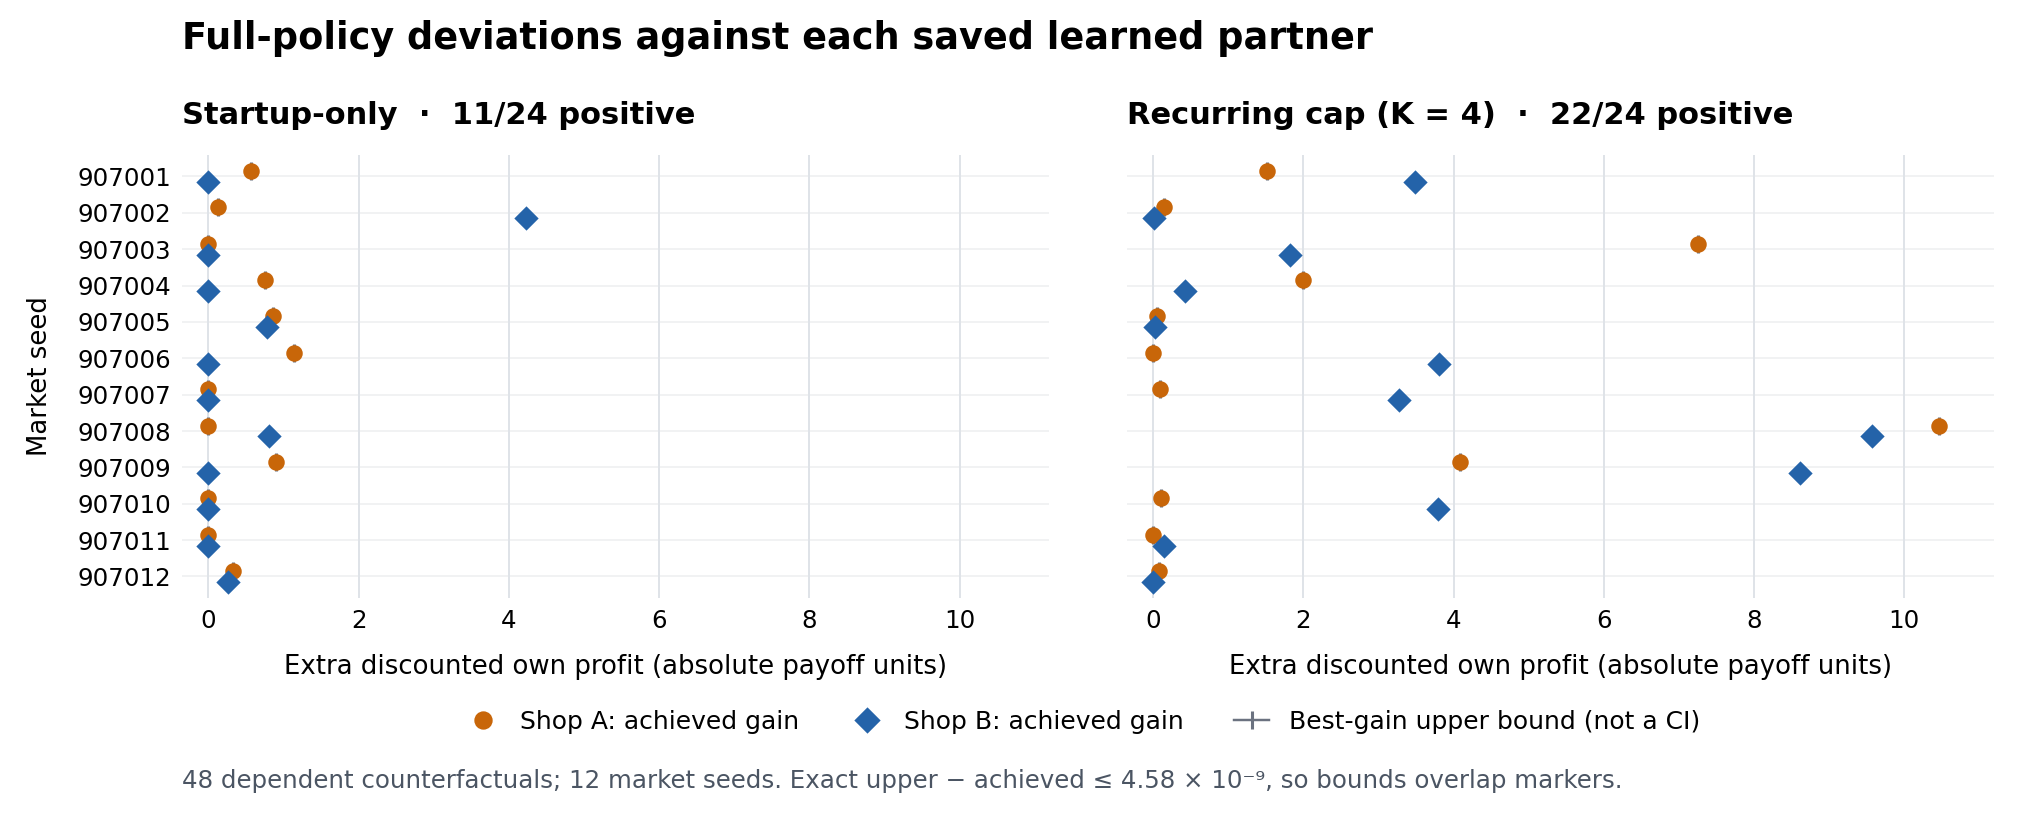
\includegraphics[width=0.94\linewidth]{images/learned-incentive-gains.png}\end{center}

\reportcaption{Figure 5. All 48 exact attained discounted-profit gains, both sellers and controllers. Seed identities are paired and dependent; whiskers show possible best-gain upper bounds, not confidence intervals. The maximum remaining response gap is below $4.58\times10^{-9}$ profit units, so the whiskers are visually indistinguishable at this scale. Zero attained gains remain visible. Gamma is mathematical 19/20; all decimals are approximate.}

\reportcaption{Table 6. Complete achieved-gain summaries in discounted profit units; exact signs, descriptive seller labels, no pooled independence.}

{\fontsize{9}{10.8}\selectfont\noindent\begin{tabular}{@{}>{\raggedright\arraybackslash}p{0.2260692\dimexpr\linewidth-48pt\relax}>{\raggedright\arraybackslash}p{0.1160896\dimexpr\linewidth-48pt\relax}>{\raggedright\arraybackslash}p{0.2057026\dimexpr\linewidth-48pt\relax}>{\raggedright\arraybackslash}p{0.1507128\dimexpr\linewidth-48pt\relax}>{\raggedright\arraybackslash}p{0.1507128\dimexpr\linewidth-48pt\relax}>{\raggedright\arraybackslash}p{0.1507128\dimexpr\linewidth-48pt\relax}@{}}\toprule
\textbf{Controller} & \textbf{Available} & \textbf{Gain + / 0 / -} & \textbf{Minimum} & \textbf{Median} & \textbf{Maximum}\\\midrule
Startup, then guard & 24/24 & 11 / 13 / 0 & 0.000000 & 0.000000 & 4.226564\\
Recurring K=4 & 24/24 & 22 / 2 / 0 & 0.000000 & 0.971166 & 10.459687\\
\bottomrule\end{tabular}\par}\vspace{3pt}

{\fontsize{9.4}{11.6}\selectfont All 48 responses meet the prospective $10^{-6}$ absolute gap target. Largest relative attained gains are about 0.896\% of baseline discounted profit for startup and 2.355\% for K=4: useful but modest. All baseline/response paths have exactly zero discounted exposure to originally unvisited states or never-tried chosen actions for either firm. This removes that particular explanation of these attained gains, not every off-path or learning concern.\par}

{\fontsize{9.4}{11.6}\selectfont Customer benefit and private gain are separate. Response-cycle customer benefit falls in 16/24 K=4 cases, rises in 6 and is unchanged in 2; startup gives 11 rises and 13 unchanged. These are eventual-cycle means, not discounted welfare or finite-prefix guarantees. A profitable allowed response does not invalidate the all-policy welfare floor or prove collusive intent. The earlier 96-label fixed-script audit remains in the evidence; its special cap-reset block simplification does not apply to learned history-dependent partners [4].\par}

\clearpage

% Source section 15: Full-grid replay, reference scope and resources

\reportheading{Appendix: Full-grid replay, scope and resources}

The reference was prospectively fixed after the matched-clock findings. V1 true administrative validation rejected omitted independent plan-metadata fields before any anchors or training. Its frozen snapshots, failed traceback and withdrawal remain preserved. V2 changes only the expected-plan parent and regression test, including direct comparison with every complete primary CLI plan. All 73 invented scientific tests and a newly source-bound maximal rehearsal pass before the accepted V2 freeze. No outcome-driven rerun, seed replacement or budget extension occurred.
\par

The new 12 runs independently replay 24M rounds from zero, 48M private updates, all 24 dense checkpoints and 2,400 distinct 10K-round transcript blocks. The earlier 24 matched runs independently replay 48M rounds; the older 192-run study still does not claim full trajectory replay. Independent full-grid anchors decode saved binary64 weights separately, retain every Nash/joint tie and add private profits exactly. Original physical masks stay hash-bound while the new later support is explicitly the full original grid. No old guard envelope or floor transfers.
\par

Primary execution: 212.049s. Full independent audit: 135.143s. Largest primary approximately paired working-set sample 258,764,800B; independent 317,091,840B. Canonical dense output 686,384,640B; stored before completion 216,926,381B; raw-equivalent 756,629,193B. All declared soft targets pass. Primary milestone sampling and independent 50ms sampling may miss peaks and are not private-memory measurements. Shared V8/Math.exp/crypto/zlib and inherited economic tables remain limitations.
\par

The first public export attempt stopped before writes because the full audit lacked a prospectively expected immutable-kernel alias present in the administrative receipt. The corrected presentation adapter retains all three mandatory source fields and binds the old kernel to its fixed accepted hash through live/snapshot/old-input closure; a present optional alias must match. Targeted tests reject missing/wrong kernel bindings. Scientific sources, receipts, Q data and numerical results were not changed or rerun.
\par

The registered final 100K exploratory-training windows also have lower full-grid customer benefit in all twelve pairs: mean difference approximately -13.312819. This distinct secondary endpoint includes exploration, does not replace the primary cycle contrast and gives no convergence guarantee.
\par

Removing support constraints changes training experience and frozen execution together. Equal allocation and rounds do not equalize legal choices or visits per action. The static simultaneous anchors do not certify dynamic learned equilibria. The 907009 profit exception is retained rather than treating high prices or aggregate profit as universal mutual benefit. All per-endpoint exact prices, individual/joint profits, support and training windows are in endpoint-metrics.csv; static ties and exact fractions are in stage-anchors.csv.
\par

{\fontsize{7.7}{9.5}\selectfont Reference manifest: research/guard-reference-results/manifest.json\\\nolinkurl{1d800d2a8bae45a0d3710de3889674fa9ed95202f5484619454242e90a34d4e3}\par}

{\fontsize{7.7}{9.5}\selectfont Reference authoritative audit: research/guard-reference-results/independent-audit.json\\\nolinkurl{2443c1f0874aac903c2125b68b47d6c7a7401d801969829b433d79a47e14bc7b}\par}

{\fontsize{7.7}{9.5}\selectfont All twelve paired reference rows: research/guard-reference-results/analysis.json\\\nolinkurl{b37ddc0cd2a2844e89700bc3097ce5b6225164db861e9952cb7f2d428f92a592}\par}

\end{document}
